% Single sided library version
\documentclass{article}

\usepackage{graphics}
\usepackage{graphicx}
\usepackage{epstopdf}
%\usepackage{pdflscape}
\usepackage{afterpage}
\usepackage{hyperref}
\usepackage{mathrsfs}

\usepackage{amsmath}

\usepackage{pgfplots} 
\pgfplotsset{compat=1.13}

\usepackage{tikzscale}
%\usetikzlibrary{external}
%\tikzset{external/force remake=true} 

\usepgfplotslibrary{external}
\tikzexternalize % activate!

\listfiles
%\usepackage[mode=buildnew]{standalone}
%\usepackage{standalone}
%\usepackage{tikz}
%\pgfplotsset{compat=newest}

\begin{document}

\section{Testing TIKZ}

\begin{figure}
  \centering
  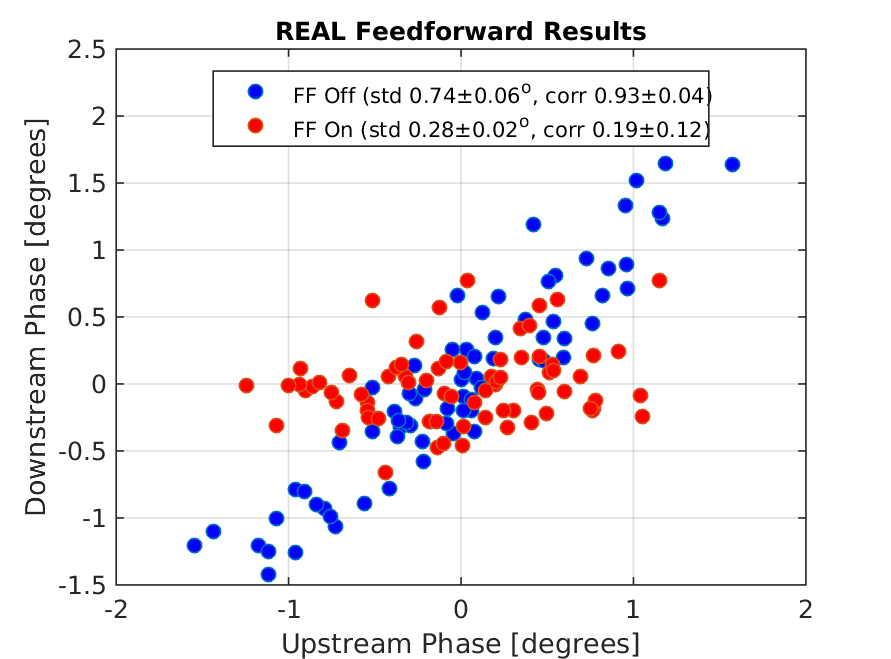
\includegraphics[width=\textwidth]{figs/BestFF_Real}
%  %\includestandalone[width=0.75\textwidth]{Figures/feedforward/BestFF_Flatness}
  \caption{Flatness of the initial (blue) and corrected (red) downstream phase along the pulse.}
  \label{f:BestFF_Flatness}
\end{figure}

%\begin{figure}
%  \includestandalone[mode=buildnew]{newtest}
%  \caption{Flatness of the initial (blue) and corrected (red) downstream phase along the pulse.}
%  \label{f:BestFF_Flatness}
%\end{figure}

sdgodfgioh

\end{document}
